\chapter{Formát PDF}
Formát \textbf{PDF} (\textbf{P}ortable \textbf{D}ocument \textbf{F}ormat) je souborový formát vyvinutý společností Adobe v roce 1992. PDF formát byl vyvinut za účelem konzistentní prezentace dokumentů (spustitelné na více zařízeních a různých platformách). Díky konzistenci lze dosáhnout toho, že PDF soubor vytvořený a uložený v systému Windows bude zobrazen totožně na systémech Mac, na všech distribucích Linuxu nezávisle na použitém PDF prohlížeči (Adobe Reader, Foxit a další).
\par 
V PDF souboru lze uchovávat velice širokou škálu dat, včetně formátovaného textu, vektorové grafiky a rastrových obrazů, nebo například informace o rozložení, velikosti a tvaru stránky. Informace definující umístění jednotlivých položek (jsou zde zahrnuty i editovací objekty pro formuláře) na stránce jsou zde uloženy též. Do dokumentu lze ukládat i metadata. Metadata jsou informace uložené v hlavičce souboru a lze do nich uložit název dokumentu, autora dokumentu, předmět a klíčová slova. Je zde možnost uložit heslo, aby byl dokument přístupný pouze autorizovaným uživatelům. Všechny tyto informace jsou uloženy ve standardním formátu \cite{PDFTechTerms, PDFWhatIs}.


\section{Objekty}
PDF Objekty jsou základním stavebním kamenem pro uchovávání dat v dokumentu. Množinou PDF objektů lze reprezentovat bitmapové a vektorové objekty, barevné prostory, text, fonty aj. \cite{PDFExplained}.
\subsection{Základní objekty}
V PDF můžeme najít celkem 5 základních objektů:
	\begin{itemize}
		\item \textbf{Celá a reálná čísla} - Celá čísla jsou reprezentována jako jedno nebo více desetinných čísel z rozsahu 0..9 se znaménkem + nebo - před číslem. Reálné číslo je celé číslo rozšířené o desetinnou část s ideálně jedním desetinným číslem (reálná čísla nelze popsat exponenciálním způsobem). Přesnost a rozsah celých a reálných čísel je definován jednotlivými implementacemi PDF. V některých implementacích platí pravidlo které přetypuje celé číslo na reálné po přesáhnutí předem daného rozsahu.
		\item \textbf{Řetězce} - Řetězec je reprezentován jako množina po sobě jdoucích bytů vepsaných mezi jednoduché závorky. Jako příklad lze uvést: \textit{(Hello, World!)}. Pro zobrazení zpětného lomítka a jednoduchých závorek je potřeba před tyto znaky přidat zpětné lomítko pro jejich správné zobrazení v dokumentu. V tabulce \ref{fig:table_escaped} lze vidět využití zpětného lomítka pro zobrazení odřádkovacích znaků:
			\begin{table}[h!]
			\centering
			\begin{tabular}{|l|l|} 
			\hline
			\textbf{Sekvence znaků}    & \textbf{Význam}                \\ 
			\hline
			\textit{\textbackslash{}n} & \textit{Line feed (LF)}        \\ 
			\hline
			\textit{\textbackslash{}r} & \textit{Carriage return (CR)}  \\ 
			\hline
			\textit{\textbackslash{}t} & \textit{Tab}                   \\ 
			\hline
			\textit{\textbackslash{}b} & Backspace                      \\
			\hline
			\end{tabular}
			\caption{Odřádkovací sekvence znaků}
			\label{fig:table_escaped}
			\end{table}
		\newline Řetězce můžou být reprezentovány i jako sekvence hexadecimálních čísel vložených mezi znaky \textbf{<} a \textbf{>}. 
		\newline Jako příklad lze uvést: \textit{<4F6EFF00> \textrightarrow 0x4F, 0x6E, 0xFF, 0x00}.

		\item \textbf{Jména} - Jméno je reprezentováno jako sloučení zpětného lomítka a řetězce (př. \textit{/Jmeno}). Za jméno se pokládá i zpětné lomítko bez řetězce. Pokud bychom potřebovali nadefinovat v dokumentu jméno, jenž bude obsahovat mezery, musíme do řetězce přidat i sekvenci znaků \textbf{\#20}, jelikož v ASCII tabulce je hexadecimální hodnota 20 vyjádřena jako prázdný znak. Jména jsou case-sensitive, proto \textit{/Jmeno} a \textit{/jmeno} jsou rozdílná jména. Jeho využití v PDF je prosté, slouží jako klíče ve slovnících a pro definice složitějších (vícehodnotových) objektů.
		\item \textbf{Boolean (pravdivostní) hodnoty} - Logické hodnoty \textbf{true}/\textbf{false} a vyskytuje se v jednotlivých záznamech ve slovníku jako příznak.
		\item \textbf{Hodnota null} - Nabývá hodnot \textit{f} (free) nebo \textit{n} (use) a vyjadřuje, zda je objekt vyobrazen v dokumentu.
	\end{itemize}
\subsection{Složené objekty}	
Složený objekt je takový objekt, který obsahuje seřazenou/neseřazenou množinu základních objektů i množinu složených objektů.
	\begin{itemize}
		\item \textbf{Pole} - Pole je v PDF reprezentováno jako seřazená množina základních i složených PDF objektů (v poli může být uložen například i slovník nebo pole) nezávisle na typech (v poli lze uchovávat například řetězec a číslo zároveň). Hodnoty pole jsou vloženy mezi znaky \textbf{[} a \textbf{]}.
		\item \textbf{Slovníky} - Slovník se skládá z množiny dvou hodnot: klíče a hodnoty, pomocí kterých se slovník namapuje. Klíč je reprezentován pomocí \textbf{jména}, zatímco hodnota může být kterýkoliv PDF objekt, povoleny jsou i slovníky nebo pole. Slovníky jsou uloženy mezi znaky \textbf{<<} a \textbf{>>}.
		\item \textbf{Datové proudy} - Datové proudy slouží především pro uložení binárních dat a skoro ve všech případech jsou zkomprimovány různými kombinacemi algoritmů, které jsou popsány v kapitole \ref{komprese}, proto datové proudy musí být zároveň i nepřímým odkazem. Skládají se ze slovníků a části binárních dat. Slovník je využit pro ukládání parametrů binárních dat, jako například délka binárních dat aj.
	\end{itemize}
\subsection{Linkovací objekty}
PDF objekty můžou být různě velké. Pokud je objekt až příliš veliký, pak jsou v kódu dokumentu využity nepřímé odkazy. Na obrázku \ref{fig:indirect_reference} si lze všimnout využití nepřímých odkazů ve slovníku. 
	\begin{figure}[h!]
	\centering
	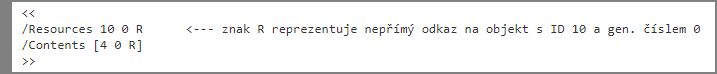
\includegraphics[width=12cm]{img/pdf_indirect_reference}
	\caption{Ukázka nepřímého odkazu}
	\label{fig:indirect_reference}
	\end{figure}

\section{Komprese dat v PDF}
\label{komprese}
PDF soubory moho být poměrně kompaktní, o mnoho menší než ekvivalentní postscriptové soubory. Tato vlastnost je dosažena nejen lepší strukturou dat, ale i díky kompresním algoritmům, které jsou velice efektivní. Typ komprese dat PDF souboru lze zjistit pomocí textového editoru, který dokáže zpracovat binární data, vyhledáním klíčového slova \textbf{/Filter}. Níže jsou popsány kompresní algoritmy využívané v PDF \cite{PDFPrepressure}.
\begin{itemize}
	\item \textbf{CCITT G3/G4} - Algoritmus je bezeztrátový a využívá se pro vykreslení černobílých obrázků.
	\item \textbf{JPEG} - JPEG algoritmus může být jak ztrátový, tak i bezeztrátový. V Acrobatu se využívá pouze ztrátový s 5 stupni komprese. Využívá se pro barevné a šedotónové obrázky.
	\item \textbf{JPEG2000} - Rychlejší algoritmus na bázi JPEGu. Víceméně se nepoužívá, jelikož není kompatibilní se staršímy systémy a vysokýmy nároky na procesor.
	\item \textbf{Flate} - Bezeztrátový algoritmus, vychází z kompresních algoritmů LZ77 a Huffmanova kódování.
	\item \textbf{JBIG2} - Alternativní k CCITT. V Dnešní době se nevyužívá z důvodu pomalejší komprese než je u jeho protějšku.
	\item \textbf{LZW} - Komprimací LZW algoritmem lze dosáhnout až o polovinu menší velikosti díky komprimaci veškerého textu a operátorů v souboru.
	\item \textbf{RLE} - Bezeztrátový algoritmus pro vykreslování černobílých obrázků. Nahrazen efektivnějším algoritmem CCITT.
	\item \textbf{ZIP} - Bezeztrátový algoritmus, učinější než jeho protějšek LZW.
\end{itemize}

\section{Vnitřní struktura PDF}
Vnitřní reprezentace PDF souboru je rozdělena na sekce, které jsou znázorněny na obrázku \ref{fig:pdf_internal_structure}.

\begin{figure}[h!]
\centering
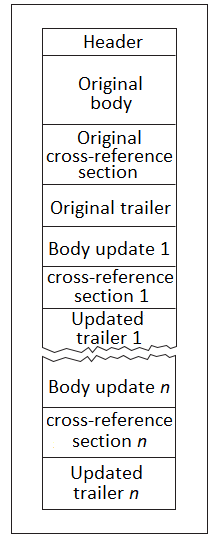
\includegraphics[width=4cm]{img/pdf_internal_structure}
\caption{Interní struktura PDF souboru}
\label{fig:pdf_internal_structure}
\end{figure}

Z obrázku lze vyčíst, že se zde vyskytují 4 hlavní sekce: \textit{Header, Body, Cross-reference a trailer}. Díky jedné z vlastností PDF formátu se při úpravě souboru staré sekce neodstraní, místo toho se pouze na jeho konci vytvoří nové sekce \cite{PDFInfoSec}.
\begin{itemize}
	\item \textbf{Header} - Hlavička souboru je uložena na první řádce, obsahující primárně použitou verzi PDF.
	\begin{figure}[h!]
	\centering
	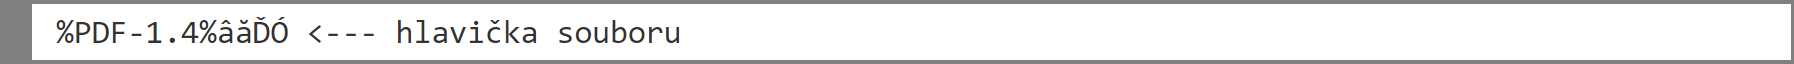
\includegraphics[width=12cm]{img/pdf_hlavicka}
	\caption{Ukázka hlavičky}
	\label{fig:pdf_header}
	\end{figure}
	
	\item \textbf{Body} - V těle dokumentu jsou uložena veškerá data objektů reprezentující celý dokument. Objekty jsou referencovány v tabulce Cross-reference z důvodu rozprostření částí dat patřících k danému objektu po celé sekci.Pokud se v dokumentu vyskytuje jeden obrázek/zvukový záznam vícekrát než jednou, tak se poté všechny objekty reprezentující obrázky odkazují na jedny data \cite{PDFAdobe}.
	\begin{figure}[h!]
	\centering
	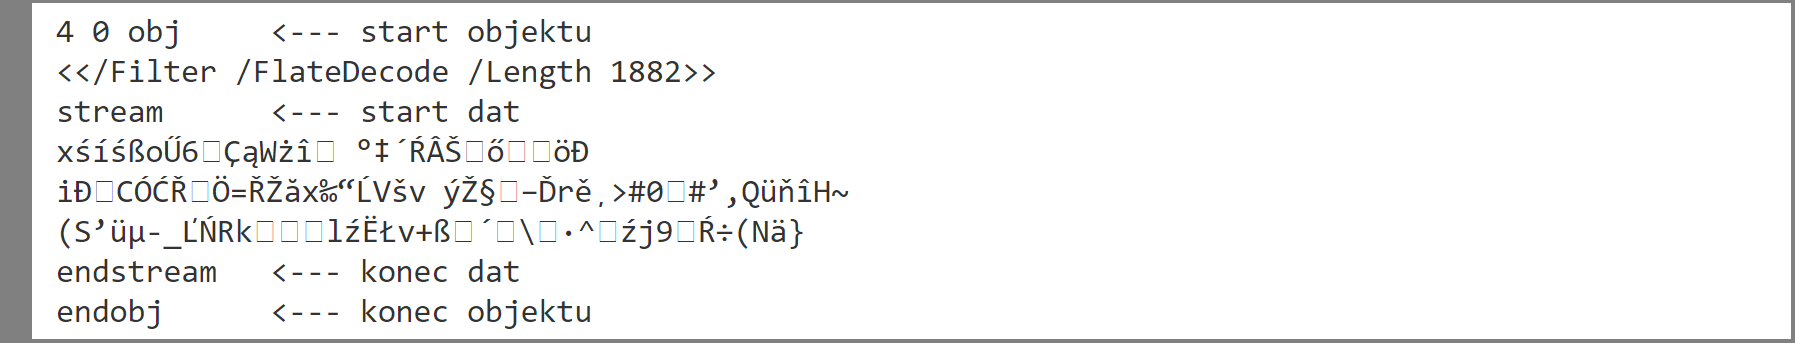
\includegraphics[width=12cm]{img/pdf_body}
	\caption{Ukázka dat objektu}
	\label{fig:pdf_body}
	\end{figure}

	\item \textbf{Cross-reference table} - Jinak nazývána \textbf{xref} je tabulka obsahující reference na veškeré objekty uložené v těle a v kódu začíná řetězcem \textit{xref}. Reference uložená v tabulce je reprezentována na 2 řádcích pomocí řetězce a skládá se z 5 částí o celkové velikosti 20 bytů včetně oddělovačů \textit{CRLF}:
	\begin{itemize}
		\item \textit{Číslo objektu} - Jednoznačný číselný identifikátor objektu.
		\item \textit{Počet subobjektů} - Počet částí daného objektu vyskytujícího se v dokumentu.
		\item \textit{Začátek objektu} - Tvoří většinu řetězce (prvních 10 bytů) a určuje offset od začátku PDF dokumentu až po začátek daného objektu.
		\item \textit{Generační číslo objektu} - Vyjadřuje jak často byl objekt vymazán při úpravě dokumentu. 
		\item \textit{Identifikátor využití} - Nabývá hodnot \textit{f} (free) nebo \textit{n} (use) a vyjadřuje, zda je objekt vyobrazen v dokumentu.
	\end{itemize}
	\newpage
	\begin{figure}[h!]
	\centering
	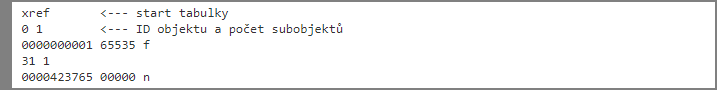
\includegraphics[width=12cm]{img/pdf_xref}
	\caption{Ukázka jednoduché xref tabulky}
	\label{fig:pdf_xref}
	\end{figure}

	\item \textbf{Trailer} -  Trailer je seznam informací, ze kterých lze snadno zjistit například velikost nebo umístění xref tabulky. Trailer může obsahovat tyto elementy:
	\begin{itemize}
		\item \textit{Size} - Udává počet objektů referencovaných v xref tabulce. 
		\item \textit{Prev} - Offset od začátku dokumentu k předchozí xref tabulce.
		\item \textit{Root} - Odkazuje na objekt obsahující informace ohledně katalogu xref tabulek.
		\item \textit{Encrypt} - Specifikuje komprimující algoritmus použití pro daný dokument.
		\item \textit{Info} - Obsahuje dodatečné informace ohledně katalogu xref tabulek.
		\item \textit{ID} - 2-bytový identifikátor PDF dokumentu.
		\item \textit{XrefStm} - Offset od začátku dokumentu až k dekódovanému xref streamu. Využívá se pouze u hybridně-referencovaných souborů pouze tehdy, kdy hledaný objekt není nalezen v xref tabulce (před tím, než se volá element \textit{Prev}). 
	\end{itemize}
	\begin{figure}[h!]
	\centering
	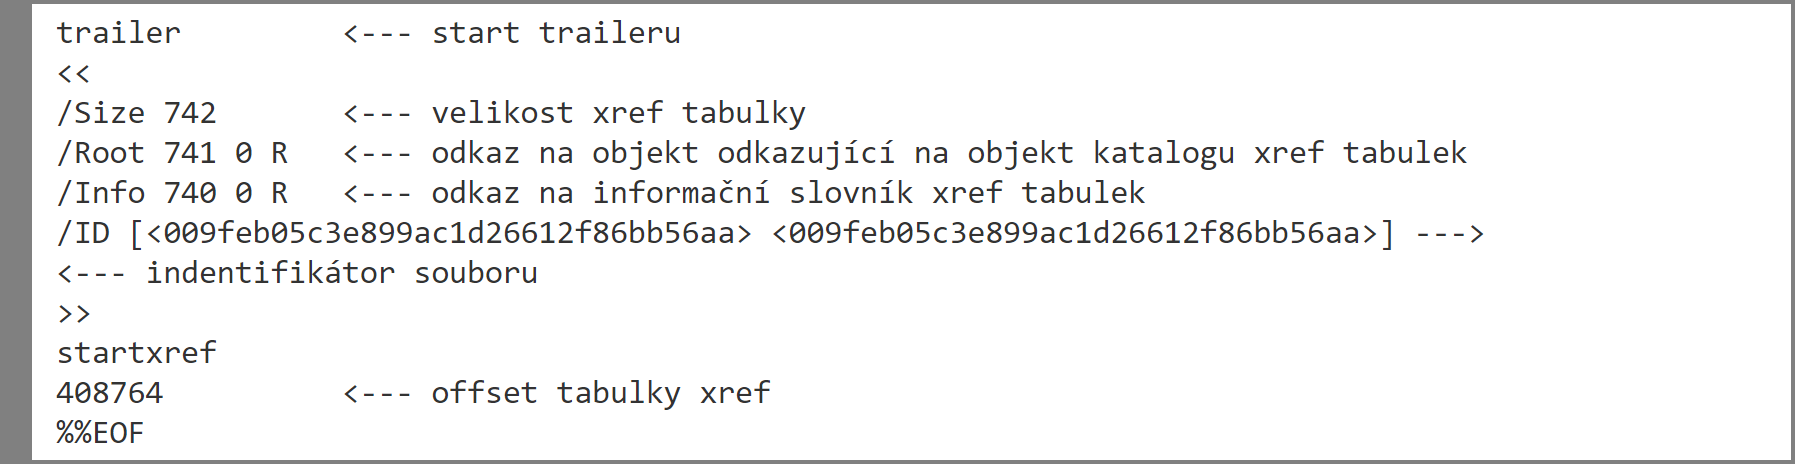
\includegraphics[width=12cm]{img/pdf_trailer}
	\caption{Ukázka traileru}
	\label{fig:pdf_trailer}
	\end{figure}
\end{itemize}
\section{Formuláře v PDF}